\documentclass[
  11pt
 ,abstracton
 ,parskip=full
 ,toc=bibliography
 ,toc=listof
 ,ngerman
]{scrreprt}
% abstracton        adds abstract to document
% parskip           insert space between paragraphs
% toc=bibliography  adds bibliography to toc
% toc=index         ...
% toc=listof        adds figures to toc
% ngerman           option for babel and cleveref

%--------------------------------------
% Packages
%--------------------------------------
% Encoding
\usepackage[utf8]{inputenc}
\usepackage[T1]{fontenc}

% https://en.wikibooks.org/wiki/LaTeX/Paragraph_Formatting#Multiline_comments
\usepackage{verbatim}

% KOMA Script
% -----------
% suppress: 'Class scrreprt Warning: \float@addtolists detected!'
\usepackage{scrhack}

% Header & Footer
\usepackage{myheader}

% German-specific commands
\usepackage{babel}
\usepackage{csquotes}

% Use href and url
\usepackage{hyperref}
\usepackage{cleveref}

\usepackage{graphicx}
\graphicspath{ {./img/} }

% Bibliography
% https://en.wikibooks.org/wiki/LaTeX/Bibliography_Management
\usepackage[backend=biber,
            %style=numeric-comp,
            citestyle=numeric-comp,
            sortcites=true]{biblatex}
\addbibresource{bib/library.bib}
\nocite{*}

% Source Code Listings
\usepackage{listings} 
\usepackage{mylist}

\usepackage{tabu}
% for noitemsep
\usepackage{enumitem}

% Math, Theorems etc.
% -------------------
%\usepackage{amsmath, amsthm, amssymb}
%\everymath{\displaystyle}

%--------------------------------------
% Meta
%--------------------------------------

% Titelblatt: Name, Titel, Datum (Abgabetermin oder Semester),
% Studiengang und Kurs, Hochschule
\titlehead{ZHAW - Zürcher Hochschule für angewandte Wissenschaften}
\subject{Seminararbeit}
\title{Information Retrieval}
\subtitle{ Evaluierung der Retrieval-Leistung einer Search\\
           Engine am Beispiel einer Media Library }
        
\author{
  Michael Kressibucher\\
  %\texttt{kressmic@students.zhaw.ch}
  \texttt{\href{mailto:kressmic@students.zhaw.ch}{kressmic@students.zhaw.ch}}
}

\date{
    Betreuerin: Ruxandra Domenig\\
    %Stand:    \today\\
    Abgabe:   15. Juni 2016
}

%--------------------------------------
% Document
%--------------------------------------
% Only includes following files
% includeonly does not mess up aux file and retains
% references.
\includeonly{
  %tex/00_exercise,
  tex/10_intro,
  tex/15_media_formats,
  tex/20_setup,
  tex/30_analysis,
  tex/60_conclusion,
}
\begin{document}
\maketitle

\begin{abstract}
  In dieser Arbeit wird mit Apache Lucene ein
Index von Mediadateien im MP3 und FLAC Format erstellt.
Die notwendigen Metadaten werden mit der
Apache Tika Library von den Dateien extrahiert.
Vom erstellten Index wird appliaktorisch eine
Abfrage erstellt. Für die anschliessende Analyse
des Index werden die Abfragen mit Luke, einem
Index Analyse Tool, ausgeführt. Da die
Konfiguration und Abfragen an das Information
Retrieval System nicht komplex sind, sind
die Abfragen von sehr hoher Genauigkeit
mit einer guten Trefferquote.
\end{abstract}

\tableofcontents
\newpage

\chapter{Aufgabenstellung}
\paragraph{Ausgangslage} \hfill \\
Auf einem privaten Network Attached Storage (NAS) sind mehrere Hundert Video und mehrere Tausend Musikdateien abgelegt. Diese sind in groben Ordnerstrukturen organisiert. Clientseitig existiert eine Suche, mit welcher die Dateinamen durchsucht werden können. Da die meisten dieser Dateien mit Metadaten versehen ist es wünschenswert auch diese Daten durchsuchen zu können.

\paragraph{Ziel der Arbeit} \hfill \\
Im Rahmen dieser Arbeit sollen die Metadaten der Dateien einer Media Library auf einem Network Attached Storage indiziert werden. Auf dem erstellten Index sollen Suchabfragen ausgeführt werden können.

\paragraph{Aufgabenstellung} \hfill \\
\begin{itemize}
    \item Vorbereiten der Suche
        \begin{itemize}
            \item Es sollen mögliche Medienformate untersucht werden.
        \end{itemize}
    \item Aufsetzen der Suche
        \begin{itemize}
            \item Indizieren von ein bis zwei der untersuchten Medienformaten.
            \item Suchabfragen erstellen.
        \end{itemize}
    \item Analysieren der Suchabfragen
        \begin{itemize}
            \item Testdaten bestimmen.
            \item Qualität der Suche anhand von Precison und Recall mit den Testdaten bestimmen.
        \end{itemize}
\end{itemize}

\paragraph{Erwartete Resultate} \hfill \\
\begin{itemize}
    \item Analyse der möglichen Medienformate und Entscheid für ein bis zwei Formate für die Indizierung.
    \item Ein lauffähige Instanz von Lucene.
    \item Vorbereitung der Dokumente (Mediadateinen) um die Metadaten zu extrahieren.
    \item Definition von Beispiel-Anfragen und den dazu erwarteten Antworten.
    \item Analyse der Resultate.
\end{itemize}

\begin{comment}
\paragraph{Ausgangslage} \hfill \\
Auf einem privaten Network Attached Storage (NAS) sind mehrere Hundert Video und mehrere Tausend Musikdateien abgelegt. Diese sind in groben Ordnerstrukturen organisiert. Clientseitig existiert eine Suche, mit welcher die Dateinamen durchsucht werden können. Da die meisten dieser Dateien mit Metadaten versehen ist es wünschenswert auch diese Daten durchsuchen zu können.

\paragraph{Ziel der Arbeit} \hfill \\
Im Rahmen dieser Arbeit sollen die Metadaten der Dateien einer Media Library auf einem Network Attached Storage indiziert werden. Auf dem erstellten Index sollen Suchabfragen ausgeführt werden können.
\end{comment}


\chapter{Einleitung}
Im Rahmen dieser Arbeit werden Metadaten spezifischer Mediadateien
mit der Information Retrieval Bibliothek Apache Lucene 
\cite{web:lucene} indiziert und durchsucht.

Dafür werden in \cref{ch:formats} verfügbare Mediaformate und 
insbesondere deren
Metadaten genauer untersucht. In dieser Analyse werden
die zu indizierenden Attribute der Mediaformate ausgewählt.
Zusätzlich wird aufgezeigt, wie die Metadaten der Mediadateien
mit der Inhalt Erkennungs und Analyse Library Apache Tika
\cite{web:tika} aufbereitet werden.

Anschliessend werden die extrahierten Metadaten in \cref{ch:setup}
mittels Apache Lucene indiziert. Über die indizierten Attribute
wird eine erste einfache Abfrage erstellt. Primär soll der Index
verwendet werden um in \cref{ch:analysis} aus einer kleinen Menge von Dokumenten die Genauigkeit und Trefferquote von Abfragen an
den Index zu untersuchen.

Der gesamte Sourcecode zu dieser Arbeit und weitere hilfreiche
Beispiele sind unter \url{https://github.com/kressi/search-media}
verfügbar. Die Beispiele wurden alle mit
\href{http://www.scala-lang.org/documentation/}{Scala} geschrieben.
Scala ist eine Funktionale Programmiersprache welche in 
der Java Virtual Machine (JVM) ausgeführt wird. Das heisst,
alle in der Arbeit verwendeten Java Packages können ohne
weiteres verwendet werden.

\paragraph{Ausgangslage} \hfill \\
In der zu indizierenden, privaten Media Library befinden sich
Musik- und Videodateien in unterschiedlichen Formaten.
Im Rahmen dieser Arbeit werden wir daraus zwei unterschiedliche
Audioformate auswählen und indizieren.
Diese Library liegt auf einem Network Attached Storage (NAS)
und wird im lokalen Netzwerk den Clients zur verfügung
gestellt. Bei den Clients ist das NAS über das WebDAV
Protokoll unter einem lokalen Laufwerk geladen, der Zugriff
auf die Dateien geschieht also wie wenn die Dateien auf
der lokalen Festplatte gespeichert wären. Der Index wird nur
lokal für einen Client erstellt.

\begin{comment}
Vorbereiten der Suche
\begin{itemize}
    \item Es sollen mögliche Medienformate untersucht werden.
\end{itemize}

\paragraph{Result} \hfill \\
Analyse der möglichen Medienformate und Entscheid für ein bis zwei Formate für die Indizierung.
\end{comment}


\chapter{Metadaten Aufbereiten}
\label{ch:formats}

In der Media Library sind MP3 und FLAC Dateien weitaus
am häufigsten vorhanden, weshalb wir nur diese beiden Audioformate
genauer betrachten werden. Aus den Metadaten dieser
Audioformate interessiert uns vor allem das Tag, die
Metadaten zum Audio Track, wie der Interpret, der Titel
oder das Album.

Um die Metadaten der Mediadateien zu betrachten und
zu editieren, verwenden wir der Einfachheit halber das Tool
EasyTAG \cite{web:easytag}. Dieses Tool ist verfügbar für
Linux und weitere Platformen, es ist intuitiv zu bedienen.
Neben den Attributen sehen wir darin zum Beispiel in
\cref{fig:easytag} auch, dass die Metadaten der gewählten
Datei als  Vorbis Tag gespeichert sind.

\begin{figure}[ht]
    \centering
    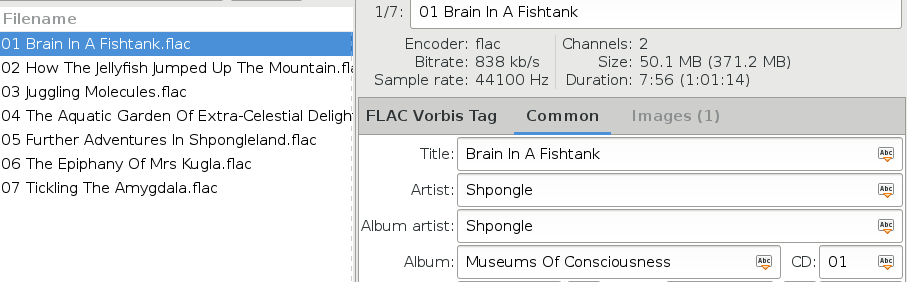
\includegraphics[width=\textwidth]{easytag}
    \caption{Metadaten mit EasyTAG editieren}
    \label{fig:easytag}
\end{figure}

\section{MP3 Format}
MPEG-1 oder MPEG-2 Audio Layer {III} allgemein bekannt als MP3
ist ein verlustbehafteteter Audio Codec. Die
\href{http://mpeg.chiariglione.org/}{Movie Pictures Expert Group}
(MPEG) hat dieses Format entworfen.
MP3 Dateien können aus mehreren Frames bestehen, ein
solches Frame enthält jeweils einen MP3 Header und MP3 Daten.
Der Header enthält Informationen wie zum Beispiel das Format,
die Version des Formates oder die Bitrate. Der MP3 Standard
enthält offiziell keinen Container für Tags. Üblicherweise werden
Tags im ID3v1 oder ID3v2 Format an MP3 Dateien gehängt.
ID3v1 ist ein \(128\) Byte langer Block welcher wie in 
\cref{tab:id3v1}
aufgebaut ist. Dieser Block enthält minimale Metadaten
über das in der MP3 Datei gespeicherte Stück.

\begin{table}[ht]
    \centering
    \begin{tabu}{l|l|l}
        \hline
        \rowfont[c]{\bfseries} Feld & Bytes & Beschreibung \\
        \hline
        header    & 3           & "TAG" \\
        title     & 30          & \\
        artist    & 30          & \\
        album     & 30          & \\
        year      & 4           & \\
        comment   & 28 oder 30  & Optional, letzte 2 Bytes für Track Nr. \\
        zero-byte & 1           & Enthält 0, falls Track Nr. vorhanden \\
        track     & 1           & Track Nr. falls zero-byte gesetzt \\
        genre     & 1           & Index in einer Liste möglicher Genres, sonst 255
    \end{tabu}
    \caption{ID3v1 Layout}
    \label{tab:id3v1}
\end{table}

Im Gegensatz zu ID3v1 hat der ID3v2 keine fixe, sondern eine
variable Länge. In einem ID3v2 können sehr viel mehr Attribute
gespeichert werden, es existiert selbst für Bildcover ein
Attribut. \cite{wiki:mp3,wiki:id3}

\section{FLAC Format}
Free and Lossless Audio Codec (FLAC) ist ein verlustfreier
Audio Codec. FLAC ist ein offenes Format und steht unter
der \href{http://www.gnu.org/licenses/gpl.html}{GNU General Public License}.
Die grundlegende Struktur einer FLAC Datei ist wie folgt aufgebaut.
\cite{web:flac}

\begin{itemize}[noitemsep]
    \item \emph{flac} als String
    \item Block mit Metadaten zu Samplerate, Anzahl Channels etc.
    \item Keinen oder mehrere Metadaten Blocks, ein Block kann ein Bild, Vorbis Kommentar oder Track Informationen enthalten.
    \item Eines oder mehrere Audioframes.
\end{itemize}

Der Standard sieht den Vorbis Comment für die Tag Metadaten vor.
Dieser Standard lässt zu, bis zu \(2^{24}\) Bytes in einem
Vorbis Comment zu speichern. Die Daten sollen in
menschenlesbarem Format gespeichert werden, damit entfallen
Probleme wie zum Beispiel das Genre im ID3 Tag Format,
welches nur als Index gespeichert wird. Um aus diesem
Index das Genre zu erhalten, muss man die überall gleiche
Liste aller Genres kennen. \cite{web:vorbiscomment}

\section{Metadaten Parsen}
\label{sec:parse}
Um die Metadaten zu den unterschiedlichen Audioformaten
zu parsen wird die Library Apache Tika \cite{web:tika}
verwendet. Diese Library bietet für verschiedenste
Dokumente, darunter Textdokument, Source Code Dateien
oder eben auch Media Dateien, Parser um aus den Dateien
Metainformationen zu extrahieren.\cite{web:tikaformats}

Mit dem \href{https://tika.apache.org/1.13/api/org/apache/tika/parser/mp3/Mp3Parser}{MP3Parser}
können Metadaten aus MP3 Dateien
extrahiert werden. Für FLAC Dateien existiert der
externe \href{https://github.com/Gagravarr/VorbisJava/blob/master/tika/src/main/java/org/gagravarr/tika/FlacParser.java}{FlacParser}
aus dem \href{https://github.com/Gagravarr/}{Gagravarr Package}.
Tika bietet mit dem
\href{https://tika.apache.org/1.13/api/org/apache/tika/parser/AutoDetectParser.html}{AutoDetectParser}
zusätzlich einen Parser, welcher einem den Umstand abnimmt
selbst entscheiden zu müssen, welcher Parser für eine
bestimmte Datei verwendet werden soll. Wir werden
nachfolgend nur mit diesem Parser arbeiten.

In nachfolgenden Listing sehen wir wie wir den Parser
verwenden um damit die \emph{metadata} aus dem
\emph{file} zu extrahieren.

\begin{lstlisting}[style=myScalastyle]
val metadata = new Metadata
val handler  = new BodyContentHandler
val context  = new ParseContext
val parser   = new AutoDetectParser
val stream   = Try(new FileInputStream(file))

stream.map( s =>
    catching(classOf[TikaException],
             classOf[SAXException])
    andFinally(s.close())
    withTry(parser.parse(s, handler, metadata, context))
) match {
    case Success(_) =>
        return metadata
    case Failure(e:Throwable) => println(e.toString())
}
\end{lstlisting}

\begin{table}[ht]
    \centering
    \begin{tabu}{l|l}
        \hline
        \rowfont[c]{\bfseries} Attribut & Wert \\
        \hline
        xmpdm:genre            & Hardstyle \\
        x-parsed-by            & org.apache.tika.parser.DefaultParser \\
        creator                & Showtek \\
        xmpdm:album            & Today is Tomorrow \\
        xmpdm:tracknumber      & 05 \\
        xmpdm:releasedate      & 2007 \\
        meta:author            & Showtek \\
        xmpdm:artist           & Showtek \\
        dc:creator             & Showtek \\
        xmpdm:audiocompressor  & MP3 \\
        title                  & FTS \\
        xmpdm:audiochanneltype & Stereo \\
        version                & MPEG 3 Layer III Version 1 \\
        xmpdm:audiosamplerate  & 44100 \\
        channels               & 2 \\
        dc:title               & FTS \\
        author                 & Showtek \\
        xmpdm:duration         & 165467.921875 \\
        content-type           & audio/mpeg \\
        samplerate             & 44100
    \end{tabu}
    \caption{Metadaten einer MP3 Datei}
    \label{tab:tikameta}
\end{table}

Die Metadaten zu einer von unseren Audiodateien
sehen wir in \cref{tab:tikameta}.
Unter diesen Attributen fällt auf, dass viele mit
\emph{xmpdm} beginnen. Bezeichner vor dem Doppelpunkt
sind Formate in welchen Tika dieses Attribut ablegt.
\emph{xmpdm} steht für XMP Digital Media.
Extensible Metadata Platform (XMP)
ist ein Standard für den Austausch von Metadaten.\cite{wiki:xmp}

Im nachfolgende Kapitel werden wir die Attribute \emph{xmpdem:genre},
\emph{author}, \emph{xmpdm:releasedate}, \emph{title}
und \emph{xmpdmalbum} indizieren.
\begin{comment}
Aufsetzen der Suche
\begin{itemize}
    \item Indizieren von ein bis zwei der untersuchten Medienformaten.
    \item Suchabfragen erstellen.
\end{itemize}

\paragraph{Result} \hfill \\
\begin{itemize}
    \item Ein lauffähige Instanz von Lucene.
    \item Vorbereitung der Dokumente (Mediadateinen) um die Metadaten zu extrahieren.
\end{itemize}
\end{comment}


\chapter{Information Retrieval}
\label{ch:setup}

Im vorigen Kapitel haben wir uns die Metadaten der
zu indizierenden Dokumente angeschaut. Diese Metadaten
werden wir nun mit der Library Apache Lucene \cite{web:lucene}
indizieren und durchsuchen.

\begin{figure}[ht]
    \centering
    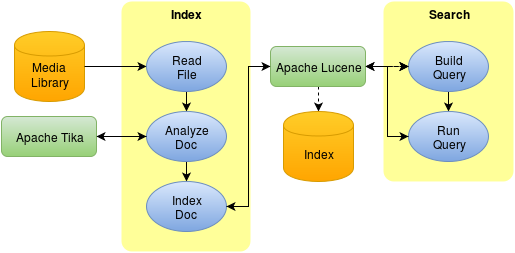
\includegraphics[width=\textwidth]{architecture-tika-lucene}
    \caption{Architektur Information Retrieval Applikation}
    \label{fig:tika-lucene}
\end{figure}

In \cref{fig:tika-lucene} sehen wir die einzelnen Elemente
welche in einer Information Retrieval Applikation mitwirken
und in welchen Schritte welche Apache Libraries verwendet
werden.
Aus dieser Übersicht wollen wir uns nun dem letzten Schritt des Erstellens
des Index zuwenden, dem Indizieren der Metadaten der Dokumente.
\cite{web:tika-lucene}

\section{Index erstellen}
\label{sec:createindex}
Die Metadaten, welche in \cref{sec:parse} gelesen
wurden, bilden pro gelesene Datei eine Menge von
Attributen mit Werten. Aus einer solchen Menge
wählen wir die gewünschten Attribute aus und 
fassen diese zusammen zu Dokumenten. Diese Dokumente
werden dem Index hinzugefügt.

\paragraph{Shared Memory in Linux} \hfill \\
Zugriffe auf den Index sollten möglichst schnell
ausgeführt werden. Am schnellsten sind diese, wenn
sich der Index im Arbeitsspeicher befindet. Da auf
Linux Systemen standardmässig das Verzeichnis
Shared Memory \emph{/dev/shm} im Arbeitsspeicher
geladen wird, werden wir den Index darin erstellen.
Es ist anzumerken, dass Dateien in diesem Verzeichnis
verloren gehen wenn das System heruntergefahren
wird.\cite{web:shm}

In folgendem Listing betrachten wir die Funktion,
mit welcher wir aus dem \emph{fileName} und den
\emph{metadata} ein Dokument erstellen. Allenfalls
vorhandene \emph{keywords} fügen wir dem Dokument als
einzelne \emph{StringFields} hinzu. Ein \emph{StringField}
ist ein String welcher als ganzes indiziert wird.
Das \emph{TextField} wird bei Leerzeichen oder anderen
Trennzeichen gesplittet und als mehrere \emph{Strings}
indiziert. Mit dem \emph{boolean} Wert \emph{Store.YES}
sagen wir, dass der Wert des indizierten Attributes
auch abgelegt werden soll. Alle Attribute welche leer
sind werden nicht indiziert. Weiter werden alle Attribute
welche nicht explizit indiziert werden verworfen.

\begin{lstlisting}[style=myScalastyle]
def mkDocument (fileName:String, metadata:Metadata): Document = {

    val fieldPat = "([a-z0-9]+):([a-z0-9]+)".r
    val xmpdmAttrs = Array("album", "releasedate", "genre")
    val doc = new Document()
    doc.add(new StoredField("file", fileName))
    
    for (key <- metadata.names()) {
        val name = key.toLowerCase()
        val value = metadata.get(key)
        if (!StringUtils.isBlank(value)) {
            name match {
                case "keywords" => 
                    for (keyword <- value.split(",?(\\s+)")) {
                        doc.add(new StringField(name, keyword, Store.YES))
                    }
                case "title" | "author" | "composer" =>
                    doc.add(new TextField(name, value, Store.YES))
                case fieldPat("xmpdm", attr) if xmpdmAttrs contains attr =>
                    doc.add(new TextField(attr, value, Store.YES))
                case _ => ()
            }
        }
    }
    doc
}
\end{lstlisting}

In einem Loop iterieren wir nun rekursiv über alle
Dateien in der Media Library, erstellen zu jeder FLAC und MP3
Datei ein Dokument und fügen dieses Dokument zum Index
hinzu.

\paragraph{Rekursiv über Dateien Iterieren} wird mit der
\emph{listFiles} Methode aus dem Apache Package
\emph{org.apache.commons.io.FileUtils} ausgeführt.
Diese Methode erlaubt auf einfache Weise rekursiv
über alle Dateien eines Verzeichnisses zu iterieren.
\cite{web:fileutils}

\section{Abfragen ausführen}
Auf dem soeben erstellten Index führen wir nun eine Abfrage
aus. Die Abfrage soll über mehrere Attribute ausgeführt
werden.

Abfragen müssen der Lucene Query Parser Syntax entsprechen.
Damit können unter anderem Proximity Searches, Range Searches
oder Fuzzy Searches ausgeführt werden, es können
zu durchsuchende Attribute festgelegt werden oder
auch einzelne Terme
miteinander verknüpft werden. \cite{web:lucenesyntax}

Für unsere Abfrage wollen wir für das Erste nur 
nach einem Begriff in mehreren Attributen suchen.
Dazu müssen wir den \emph{MultiFieldQueryParser}
verwenden. Nachfolgend parsed der \emph{parser}
einen Abfrage String und gibt eine \emph{Query}
zurück. Diese Query \emph{q} übergeben wir dem
\emph{IndexSearcher}. Von dem \emph{collector}
werden danach die gefundendenen Resultate geholt.
\cite{web:lucenedoc,web:luceneintro}

\begin{lstlisting}[style=myScalastyle]
def apply() {
    
    val indexDir = Paths.get(Config.indexPath)
    val index = FSDirectory.open(indexDir)

    // Build a Query object
    val fields = Array("album", "author", "composer", "album", "title")
    val analyzer = new StandardAnalyzer()
    val parser = new MultiFieldQueryParser(fields, analyzer)

    Try(parser.parse("Shpongle")) match {
        case Success(q) => 
            val hitsPerPage = 10
            val reader = DirectoryReader.open(index)
            val searcher = new IndexSearcher(reader)
            val collector = TopScoreDocCollector.create(hitsPerPage)
            searcher.search(q, collector)
            
            println("total hits: " + collector.getTotalHits())
            val hits = collector.topDocs().scoreDocs
            for (hit <- hits) {
                val doc = reader.document(hit.doc)
                println(doc.get("file") + "  (" + hit.score + ")")
            }
        case Failure(e) => println(e.toString())
    }       
}
\end{lstlisting}

Wie wir nun gesehen haben, erlaubt einem die Apache
Lucene Library auf einfache Weise, aus Dokumenten
einen Index zu erstellen und an diesen Abfragen zu
stellen. Im nächsten Kapitel wollen wir den so erstellten
Index der Media Library etwas genauer betrachten.

\begin{comment}
Analysieren der Suchabfragen
\begin{itemize}
    \item Testdaten bestimmen.
    \item Qualität der Suche anhand von Precison und Recall mit den Testdaten bestimmen.
\end{itemize}


\paragraph{Result} \hfill \\
\begin{itemize}
    \item Definition von Beispiel-Anfragen und den dazu erwarteten Antworten.
    \item Analyse der Resultate.
\end{itemize}
\end{comment}


\chapter{Analyse der Abfrage}
\label{ch:analysis}

Um dieses Information Retrieval System zu bewerten,
möchten wir die Precision (Genaugkeit) und den Recall
(Trefferquote) für typische Abfragen an das System
bestimmen. Um die dazu notwendigen Daten zu erheben
verwenden wir das Entwicklungs und Analyse
Tool für Lucene Indizes Luke.

\paragraph{Luke} kann unter anderem verwendet werden um Dokumente
im Index zu betrachten (\cref{fig:luke-docs}) oder
um Abfragen zu erstellen (\cref{fig:luke-search}).
\cite{web:lukeintro}
Luke \cite{web:luke} scheint vom ursprünglichen
Entwickler \citeauthor{web:luke}
nicht mehr maintained zu werden. Von \citeauthor{web:lukegit}
ist eine Version verfügbar in welcher auch Indizes
von Lucene in der aktuellen Version gelesen werden
können. \cite{web:lukegit}

\begin{figure}[h]
    \centering
    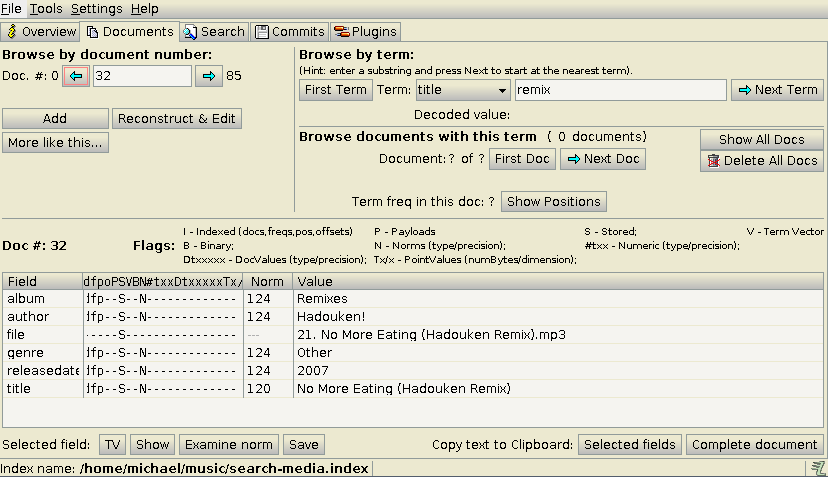
\includegraphics[width=\textwidth]{luke-documents}
    \caption{Ansicht Dokumente in Luke}
    \label{fig:luke-docs}
\end{figure}

\begin{figure}[h]
    \centering
    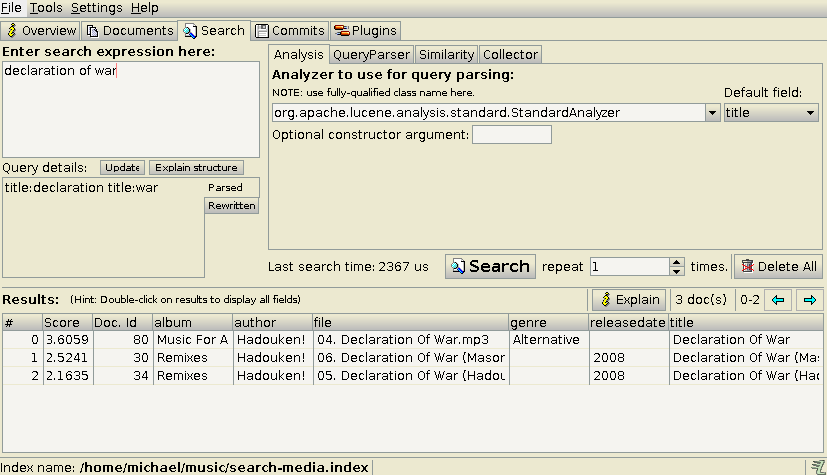
\includegraphics[width=\textwidth]{luke-search}
    \caption{Ansicht Suche in Luke}
    \label{fig:luke-search}
\end{figure}

\section{Test Daten}
\label{sec:testdata}
Damit man eine verlässliche Aussage über die Precision
und den Recall machen kann, muss man die indizierten
Dokumente genau kennen. Das heisst wir müssen genau
wissen welches die erwarteten Treffer einer Abfrage
sind.\cite[S.~152]{book:manning}

Aus der Media Library wählen wir dazu eine Menge
von \(85\) Dateien aus und erstellen einen Index,
worin nur diese Dateien indiziert werden.

\begin{table}[h]
    \centering
    \begin{tabu}{l|c}
        \hline
        \rowfont[c]{\bfseries} Abfrage & \#Resultat \\
        \hline
        *:*                               & \(85\) \\
        author:hadouken                   & \(66\) \\
        author:hadouken AND title:war     & \(3\) \\
        author:hadouken AND NOT title:war & \(63\) \\
        title:girl*                       & \(4\) \\
        title:liquid AND releasedate:2007 & \(4\) \\
        album:"museums of consciousness"  & \(7\)
    \end{tabu}
    \caption{Abfragen und Erwartete Resultate}
    \label{tab:testdata}
\end{table}

Mit den Abfragen in \cref{tab:testdata}, wollen wir ein
Spektrum von Abfragen abdecken, welches nahe am tatsächlichen
Gebrauch eines solchen Index ist. Die Anzahl
der erwarteten Results wird mit EasyTAG gezählt,
es werden dazu nicht die Dokumente in Luke betrachtet.
Damit würden allfällige Fehler, welche beim Indizieren
oder beim Abfragen mit Luke entstehen könnten,
kaschiert.


\section{Precision \& Recall}
Die vorbereiteten Abfragen führen wir nun mit Luke aus.
Von den die erhaltenen Resultate vergleichen wir dann
mit den gespeicherten Resultaten der in \cref{sec:testdata}
vorbereiteten Abfragen.

Seien \(e\) die erwarteten Resultate und \(r\)
das erreichte Resultat. Dann sind die Precision und
dre Recall wie folgt definiert.

\begin{description}
    \item [Recall] Die Fähigkeit die erwarteten Resultate zu liefern. \(r = \frac{|r \cap e|}{|e|}\)
    \item [Precision] Die Korrektheit der gelieferten Resultate. \(p = \frac{|r \cap e|}{|r|}\)
\end{description} \cite[S.~63]{book:heinrich}

\begin{table}[h]
    \centering
    \begin{tabu}{l|c|c|c|c|c}
        \hline
        \rowfont[c]{\bfseries} Abfrage & \(|r|\) & \(|e|\) & \(|r \cap e|\) & \(p\) & \(r\) \\
        \hline
        *:*                               & \(85\) & \(85\) & \(85\) & \(1\) & \(1\) \\
        author:hadouken                   & \(66\) & \(66\) & \(66\) & \(1\) & \(1\) \\
        author:hadouken AND title:war     & \(3\)  & \(3\)  & \(3\)  & \(1\) & \(1\) \\
        author:hadouken AND NOT title:war & \(63\) & \(63\) & \(63\) & \(1\) & \(1\) \\
        title:girl*                       & \(4\)  & \(4\)  & \(4\)  & \(1\) & \(1\) \\
        title:liquid AND releasedate:2007 & \(4\)  & \(4\)  & \(4\)  & \(1\) & \(1\) \\
        album:"museums of consciousness" \footnotemark  & \(0\)  & \(7\)  & \(0\)  & \(-\) & \(0\)
    \end{tabu}
    \caption{Abfragen und Erreichte Resultate}
    \label{tab:testresult}
\end{table}
\footnotetext{Diese Abfrage muss mit dem Luke XML Query Parser ausgeführt werden, in regulären Abfragen entfernt Luke \emph{of} aus dem String, so dass nur noch nach album:"museums consciousness" gesucht wird.}

Diese Resultate scheinen im ersten Moment etwas überraschend,
lassen sich jedoch erklären. Bis auf die letzte Zeile sind
jeweils genau die erwarteten Resultate erreicht worden. Dafür
gibt es unterschiedliche Gründe. Die Menge ist relativ klein,
die Wahrscheinlichkeit sinkt dadurch Ausreisser zu treffen.
Die Abfragen sind einfach, es wurden keine N-Gramme geladen,
es existieren keine Ähnlichkeitsabfragen. Dies alles sind
Features welche eine Suche in verschiedenen Bereichen für
einen Endanwender bequemer jedoch auch ungenauer  machen.

Dann ist in diesem noch das Resultate, bei welchem kein Hit
gefunden wurde. Dies liegt an der String Suche, in
\cref{sec:createindex} haben wir die meisten Attribute des
Dokuments, darunter auch \emph{album}, als \emph{TextField} 
erstellt. Ein \emph{TextField} wird in einzelne Worte aufgeteilt,
davon werden nur die einzelnen Worte indiziert, nicht der
gesamte String. Um auf diesem Feld auch eine String
Suche zu ermöglichen, könnte als mögliche Lösung ein
zusätzliches \emph{StringField} mit dem gesamten String zum Dokument
hinzugefügt werden. Dies müsste jedoch nicht auch gespeichert werden.

\chapter{Fazit}
In dieser Arbeit wurden zuerst die Formate der Mediadateien
und deren Container für Tags analysiert. Es ist interessant
die nicht geringen Unterschiede zwischen unterschiedlichen
Formaten zu erkennen. Genauso ist es spannend zu sehen,
dass ID3 Tags nicht nur für das MP3 und Vorbis Comments nicht
nur für FLAC Format verwendet werden. Sobald man jedoch damit
beginnt die Metadaten mit der Apache Tika Library zu parsen,
stellt man fest, dass zumindest im Bereich von weit verbreiteten
Mediaformaten, auch ohne jegliches Wissen über die verwendeten
Tag Container oder deren Aufbau weiterkommt. Selbst mit
Wissen über die Tag Container ist es einfacher den
\emph{AutoDetectParser} zu verwenden. Dies macht es
unglaublich leicht Metadaten aus Dateien zu extrahieren.

Als nächster Schritt wurden die Metadaten indiziert.
Auch dieser Schritt geht mit den Apache Libraries leicht von
der Hand, zumindest solange man die Standardkonfiguration verwendet.
Dies ist sehr angenehmn, so sieht man schnell
ein Resultat, was motiviert weiterzumachen. Genauso
sieht man schnell ein Resultat wenn man eine Abfrage erstellt.

Für die Analyse wurde das Tool Luke verwendet, der Funktionsumfang
dieses Tools ist für die Entwicklung und die Analyse von
Indizes unglaublich wertvoll. Um jedoch einmal erst
soweit zu kommen hat es sich erstaunlich kompliziert
herausgestellt eine Version von Luke zu finden, welche
die aktuellste Version\footnote{Zum Zeitpunkt dieser Arbeit war 6.0.0
die aktuellste stabile Version von Apache Lucene.} des
Lucene Index lesen kann. Dies mag daran liegen, dass
normalerweise \href{https://www.elastic.co/products/elasticsearch}{Elasticsearch}
oder \href{https://lucene.apache.org/solr/}{Solr} verwendet
werden, welche gleich die eigenen Analyse Tools mitliefern.
Bei der Analyse selbst wurden keine so hohe Precision und Recall
Werte erwartet. Wenn man jedoch das Information Retrieval System
betrachtet ist es logisch solche Werte zu erreichen.



\appendix

\listoffigures
\listoftables

% Bibliography
\printbibliography[title=Quellenverzeichnis]

\end{document}
%--------------------------------------
